\section{Introduction}
Millions of children around the world are born with congenital heart defects, which may require surgery to be treated. For doctors to effectively plan surgery, it is useful if a model of the heart can be 3D-printed, which requires the scans of the patient to be segmented. Traditionally, this means that an expert must manually label each voxel in the image with whether or not it belongs in the bloodpool, myocardium, or outside the heart [correct me if I'm wrong]. Currently, patient-specific 3D heart models are underused because it takes around 4-8 hours to manually segment cardiac MRI images, since each contains approximately 1503 voxels. There have been algorithms developed to segment the heart in normal adult patients, one of the most popular being atlas segmentation, which uses a fully segmented heart as a reference and tries to a patient?s heart to the given reference. However, atlas-based methods do not work well on children with congenital heart disease (CHD) due to the irregular location or shapes of the organs.

This paper proposes an alternative method to aid the segmentation of hearts with CHD. Segmenting images of hearts with CHD as opposed to healthy hearts is an additional challenge, because hearts with CHD may have incomplete or missing structures, or structures located in different areas compared to healthy hearts. Therefore, many traditional methods for segmenting these images do not work well. The method proposed in this paper attempts to address these challenges. A first step to segmentation is locating bounding boxes around the regions of interest, as there exists algorithms that will produce accurate segmentation given a bounding box of the region to be labeled.

The method proposed in this paper will localize the heart as well as structures within the heart in patients with congenital heart disease, using random forests.

\section{Related Work}
One method for segmentation of the heart in children with CHD is an interactive algorithm proposed by Danielle Pace. At each step of the algorithm, the user is directed to manually label one slice of the heart that will give the most information [1]. The algorithm then segments each target slice according to its closest reference slices. To segment a patch, the algorithm finds the k most similar patches in the set of relevant reference regions, and ``similarity" depends on patch intensities, gradients, and positions, and each pixel is labeled according to a majority vote. This algorithm greatly reduces the amount of time needed to segment a heart, but still requires user interaction.

Regression forests have also been shown to do well in image segmentation, specifically the detection and localization of organs. A. Criminisi has applied regression forests to learn the non-linear mapping from voxels directly to organ position and size [2]. The regression forest groups voxels with similar features or similar field of views together, and learns an estimate of the bounding boxes of each organ using the training data that reaches that node. Intuitively, each voxel contributes varying degrees of confidence to the estimates of the location and size of every organ. When applied on real datasets, the forest learns to recognize key indicators (such tips of the ribs or vertebrae) and those pixels provide high confidence estimates of where certain organs are located. Criminisi then compared these results against other methods, including Elastix and Simplex methods, as well as atlas methods, and showed that the regression forest method was superior in accuracy. This paper extends the regression forest methods used by Criminisi to children with CHD.

\section{Method}
\subsection{Regression Random Forests}
This paper develops a method to localize the heart in 3D MRI scans of patients with CHD, based on regression random forests. A random forest is a supervised machine learning model that consists of many decision trees, in which the training phase of each tree contains some amount of randomness. A decision tree is a flow-chart like structure in which each node is a Boolean function on the data's features. For each data point that passes through the decision tree, as it arrives at each node, the node makes a decision for whether the data point goes to its left child or right child, based on the data point's features. Figure 1 depicts a decision tree that takes in an image as input and predicts whether it was taken indoors or outdoors.

\begin{figure}
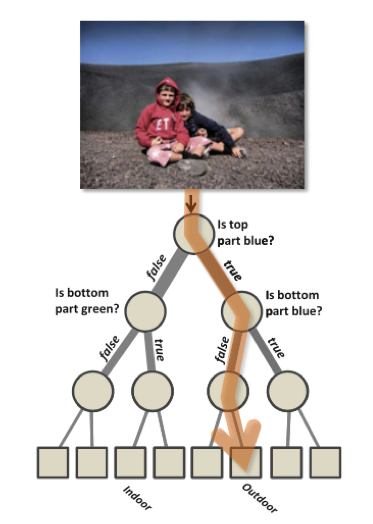
\includegraphics[scale=0.5]{decisiontree.png}
\caption{A decision tree}
\end{figure}

This paper deals with regression forests, which contain regression trees instead of decision trees. Regression trees are the same as decision trees except each leaf node contains a regression model instead of a classification model. Therefore each leaf node would predict a regression value instead of a classification label.

\begin{figure}
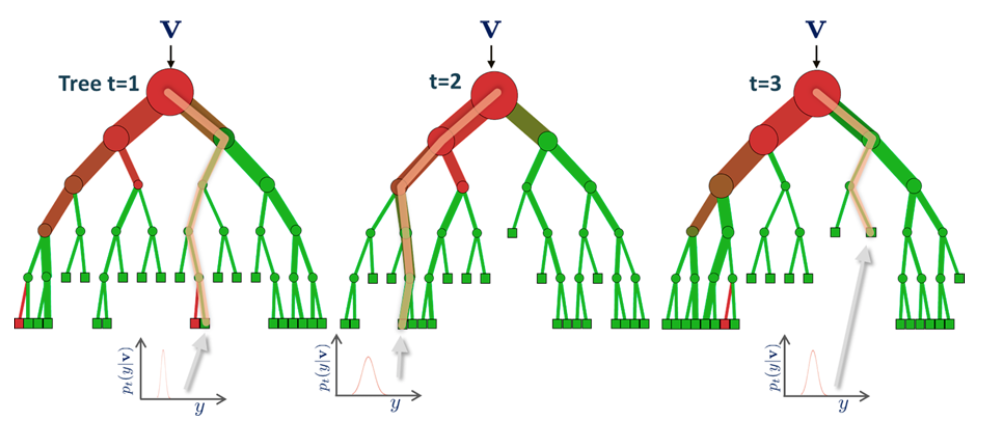
\includegraphics[scale=0.45]{regressionforest.png}
\caption{A regression forest}
\end{figure}

\begin{figure}
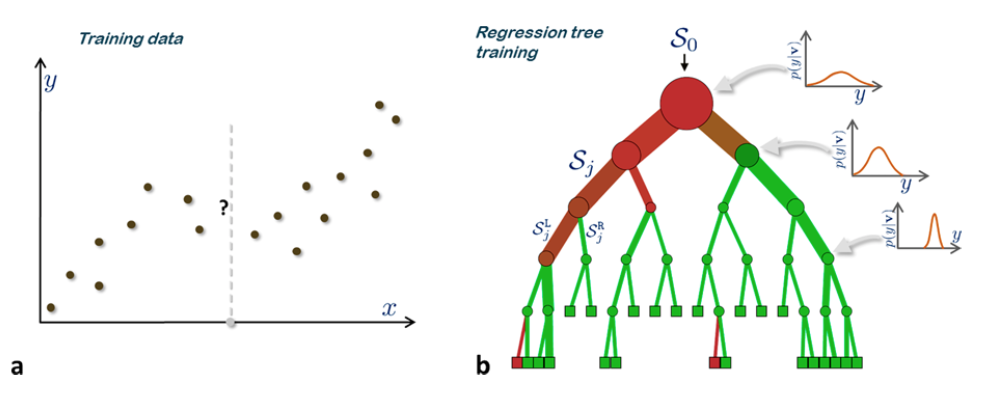
\includegraphics[scale=0.45]{regressiontraining.png}
\caption{Training a regression forest}
\end{figure}

A regression forest is produced by aggregating many regression trees. Figure 2 shows a regression forest consisting of only 3 trees, and for each tree a data point can be seen passing through the tree's branches and down to the leaf node, where it is put into a Gaussian distribution.
  
A regression forest can be trained by individually training its regression trees. Regression trees are trained by minimizing some loss function at each node. This paper uses information gain, given below:

\begin{equation}
  I(S,\theta) = H(S) - \frac{|S^L|}{|S|} H(S^L) - \frac{|S^R|}{|S|} H(S^R)
\end{equation}
where $S$ is the dataset that reaches that node, $\theta$ denotes the parameters of the function being considered at the split node, $S^L$ is the subset that will go to the left node, and $S^R$ is the subset that will go to the right node, and $H(S)$ is the entropy of a dataset $S$, given below:

\begin{equation}
  H(S) = \frac{1}{2} n \log(2\pi e  |\Sigma|)
\end{equation}

where $\Sigma$ is the covariance matrix of the Gaussian model that is fitted to the dataset at the node.

To train a regression tree, we greedily choose the split functions at each node. At each node, $K$ features are randomly selected, and the feature that maximizes the information gain given above is chosen as the split function for that node. Figure 3 depicts how a selected feature divides the training set, and then Gaussian distributions are fitted to the resulting split nodes. After each regression tree is trained, the set of these trees becomes the regression forest. The introduction of randomness in feature selection is meant to prevent overfitting: each tree is a weak learner, but the aggregation of many randomly trained weak learners should be a strong learner. Once a regression forest is trained, it can make predictions on new data points by running the data point through each of the regression trees until it reaches a leaf node, and combining the outputs of each regression tree. Training a tree terminates either when the maximum tree depth has been reached, or when the information gain is less than some threshold value.

There are three hyper-parameters that determine the structure of the regression forest: $T$ is the number of trees, $D$ is the maximum tree depth, and $K$ is the number of features being considered at each node.

\subsection{Regression Forests for Localization of the Heart}
We trained a regression forest to predict the location of the bounding box of the heart given MRI scans of patients with congenital heart disease. A bounding box is given by a 6-dimensional vector: $(x_1, x_2, y_1, y_2, z_1, z_2)$. $x_1$ and $x_2$ denote the x-values of the two faces of the bounding box that are perpendicular to the $x$-axis, where $x_1$ is the smaller of the two values, and $y_1, y_2, z_1, z_2$ are similarly defined for the other axes. Then, for each voxel that we run through the regression forest, we calculate its offset from the bounding box:
\begin{equation}
  d(\mathbf{p}, \mathbf{b}) = (x_1, x_2, y_1, y_2, z_1, z_2) - (p_x, p_x, p_y, p_y, p_z)
\end{equation}
The Gaussian model fitted at each node is then a 6D Gaussian, representing the voxel's predicted offset from the bounding box. 

To produce predictions for the bounding box of a heart given a 3D image, we take each voxel in the image and run it through the regression forest. For each voxel, we can combine the Gaussian distributions resulting from each tree in the forest by sampling the distributions. Then, we add the voxel's location to get the distribution of the predicted absolute location of the bounding box. Then, we combine the distributions from each voxel to form the predicted distribution of the absolute bounding box of the heart.

\begin{equation}
  \hat{\mathbf{b}} = \text{argmax}_{b} (\sum_{i = 0} ^ {|S|} \sum_{t=0}^{T} p(something??))
\end{equation}

%something more to say here? idk

\subsection{Feature Selection}
As mentioned previously, at each split node, $K$ features are chosen randomly for consideration as the split feature. Each feature is calculated as the mean intensity of voxels in a rectangular box, that is at some offset to the voxel. Therefore, each feature is governed by the following parameters: $\theta$ is the offset to the center of the box, which is a 3D vector, and $\phi$ is the size of the box, which is also a 3D vector. Each dimension of the box must be odd, to ensure that the center of the box is on a lattice point.

\begin{equation}
  F_{\theta, \phi} = \frac{1}{|B|} \sum_{v \in B} J(v)
\end{equation}
where $B$ is the set of voxels that lie in the box that is described by an offset of $\theta$ and a box size of $\phi$, and $J(v)$ describes the intensity at the voxel $v$. These types of features were also used by Criminisi et al.

To generate a random feature, we sample $\theta$ and $\phi$ from uniform distributions. Each element of $\theta$ is sampled from a uniform distribution from 0 to a fixed fraction of the size of the image in that dimension. Each element of $\phi$ is sampled from a uniform distribution of 1 to $2k+1$ for some $k$. We have not been able to tune parameters much, and currently the parameters are set at $\frac{1}{6}$ of the image size for $\theta$, and $k = 5$ for $\phi$. 

\subsection{Results}
Our current results are limited by the fact that the code takes a long time to run on a laptop. We are currently trying to get the code running on machines with more computing power, but there are some compiling issues on Linux that have not yet been resolved. Therefore, we have some preliminary results for very small random forests.


